\documentclass{article}

% Input packages & formatting
% Packages

% Math packages
\usepackage{amsmath} % Extended math functions
\usepackage{amssymb} % Extended math symbols (loads in amsfonts)
\usepackage{bm} % Bold math symbols
\usepackage{mathtools}

% Figure packages
\usepackage{caption} % Caption formatting for university standard
\usepackage{graphicx} % includegraphics command
\usepackage{subcaption} % Subfigures
\usepackage[section]{placeins} % Place floats in section
\usepackage{wrapfig}

% Table packages
\usepackage{booktabs} % Better tables
\usepackage{bigstrut} % Merged table cells
\usepackage{longtable} % Tables which overflow into next page
\usepackage{array}
\usepackage{colortbl} % Color table cells
\usepackage{makecell}
\usepackage{multirow}

% Fonts
\usepackage{lmodern} % Use latin modern rather than computer modern. Better for font encoding.
\usepackage[T1]{fontenc} % Allow text to be searchable in output

% Other packages
\usepackage{appendix} % Appendix environment
\usepackage{nextpage} % Cleartooddpage command
%\usepackage[square,comma,sort,numbers]{natbib} % Reference formatting
\usepackage{setspace} % Line spacing
\usepackage{listings} % Display code with syntax highlighting
\usepackage{upquote} % Vertical quotes in verbatim
\usepackage{xcolor} % Colors
\usepackage{titlesec} % Header spacing
\usepackage{xparse} % for tcolorbox
\usepackage[listings]{tcolorbox} % Colored boxes for highlighting syntax
\tcbuselibrary{breakable}
\tcbuselibrary{skins}
\usepackage{enumitem} % better enumerate/itemize options
\usepackage{fancyhdr}
\usepackage{multicol}
\usepackage{ifthen}
\usepackage{xstring}

% Table of contents
\usepackage{imakeidx} % Index page
\usepackage{tocloft} % Control of table of contents
\usepackage[nottoc]{tocbibind} % Adds bibliography, table of tables, table of figures, to table of contents
\usepackage[bookmarks,linktocpage,hidelinks]{hyperref} % Hyperlinks for sections, figures, etc.

% Formatting
% Page format
\setlength{\oddsidemargin}{0.00in}  % Left side margin for odd numbered pages
\setlength{\evensidemargin}{0.00in} % Right side margin for even numbered pages
\setlength{\topmargin}{0.00in}      % Top margin
\setlength{\headheight}{0.20in}     % Header height
\setlength{\headsep}{0.20in}        % Separation between header and main text
\setlength{\topskip}{0.00in}        % Top skip
\setlength{\textwidth}{6.50in}      % Width of the text
\setlength{\textheight}{8.50in}     % Height of the text
\setlength{\footskip}{0.50in}       % Foot skip
\setlength{\parindent}{0.00in}      % First line indentation
\setlength{\parskip}{6pt}        % Space between two paragraphs

% Captions (figures, tables, etc.)
\setlength{\floatsep}{\parskip}          % Space left between floats.
\setlength{\textfloatsep}{\floatsep}   % Space between last top float
% or first bottom float and the text
\setlength{\intextsep}{\floatsep}      % Space left on top and bottom
% of an in-text float
\setlength{\abovecaptionskip}{0.1in plus 0.25in}  % Space above caption
\setlength{\belowcaptionskip}{0.1in plus 0.25in}  % Space below caption
\setlength{\captionmargin}{0.50in}     % Left/Right margin for caption
\setlength{\abovedisplayskip}{0.00in plus 0.25in} % Space before Math stuff
\setlength{\belowdisplayskip}{0.00in plus 0.25in} % Space after Math stuff
\setlength{\arraycolsep}{0.10in}       % Gap between columns of an array
\setlength{\jot}{0.10in}                % Gap between multiline equations
\setlength{\itemsep}{0.10in}           % Space between successive items

% Counters (no section numbering)
\setcounter{tocdepth}{3}
\setcounter{secnumdepth}{0}

% Spacing
\setstretch{1.5}

\titlespacing*{\section}{0cm}{6pt}{6pt}[0cm]
\titlespacing*{\subsection}{0cm}{6pt}{6pt}[0cm]
\titlespacing*{\subsubsection}{0cm}{6pt}{6pt}[0cm]

\titleformat{\section}
{\sffamily\huge}{}{0pt}{\titlerule\vspace{-0.2cm}}
\titleformat{\subsection}
{\sffamily\itshape\Large}{}{0pt}{}

% Macro for syntax
\newtcolorbox{syntax}{
    size=small,
    sharp corners,
    colframe=black,
    colback=yellow,
    fontupper=\bfseries\ttfamily
}

% Macro for argument table
\newenvironment{args}{
    \begin{tabular}{>{\bfseries\ttfamily}p{0.25\linewidth} p{0.69\linewidth}}
    }{
    \end{tabular}\par
    \vspace{0.5\baselineskip}
}

% Note: Requires packages "listing", "xcolor", and "textcomp"
\lstdefinelanguage{verbatim}{
    basicstyle=\ttfamily\small,
    xleftmargin=9pt,
    xrightmargin=9pt,
    columns=fullflexible,
    keepspaces=true,
    breaklines=true
}

% Example code
\AtBeginDocument{
\newtcolorbox[blend into=listings]{example}[2][]{
    colback=blue!3!white,
    colframe=black,
    colbacktitle=blue!15!white,
    coltitle=black,
    sharp corners,
    enhanced,
    breakable,
    size=small,
    before upper={
        \setstretch{1.0}\lstset{language=verbatim}\vspace{3pt}\textsf{\textit{Code:}}
    },
    subtitle style={
        colback=blue!20!white,
        fonttitle=\sffamily
    },
    before lower={
        \setstretch{1.0}\lstset{language=verbatim}\vspace{3pt}\textsf{\textit{Output:}}
    },
    fonttitle=\sffamily,
    title={#2},
    #1
}
}

% Links to sub and subsub commands - optional boolean argument, default true. if false, only displays subcmd.

% Commands (and command ensembles)
\newcommand{\command}[1]{\protect\hypertarget{#1}{#1}\index{#1}}
\newcommand{\subcommand}[2]{\protect\hypertarget{#1 #2}{#1 #2}\index{#1!#2}}
\newcommand{\cmdlink}[1]{\protect\hyperlink{#1}{\textit{#1}}}
\newcommand{\subcmdlink}[3][1]{\protect\hyperlink{#2 #3}{\ifnum#1=1\relax\textit{#2 #3}\else\textit{#3}\fi}}

% Methods (first arg is class)
\newcommand{\method}[2]{\protect\hypertarget{$#1Obj #2}{\$#1Obj #2}\index{#1 methods!#2}}
\newcommand{\methodlink}[3][1]{\protect\hyperlink{$#2Obj #3}{\ifnum#1=1\relax\textit{\$#2Obj #3}\else\textit{#3}\fi}}

% Macros for figure/table names
\newcommand{\fig}{\figurename\ }
\newcommand{\figs}{\figurename s }
\newcommand{\tbl}{\tablename\ }
\newcommand{\tbls}{\tablename s }
\newcommand{\eq}{Eq. }
\newcommand{\eqs}{Eqs. }
\renewcommand{\lstlistingname}{Example}% Listing -> Example
\renewcommand{\lstlistlistingname}{List of \lstlistingname s}% List of Listings -> List of Examples
\newcommand{\ex}{Example }
\newcommand{\exs}{Examples }
\newcommand{\var}[1]{\texttt{\textbf{\$#1}}}

% Header/footer
\renewcommand{\headrulewidth}{0pt}

% Changes to hyperlinks (URLs)
\renewcommand\UrlFont{\color{blue}\rmfamily}

% New column type 
% https://tex.stackexchange.com/questions/75717/how-can-i-mix-itemize-and-tabular-environments
\newcolumntype{L}{>{\labelitemi~~}l<{}}
\newcommand{\version}{1.0.1}

\renewcommand{\cleartooddpage}[1][]{\ignorespaces} % single side
\newcommand{\caret}{$^\wedge$}

% Other macros
\renewcommand{\^}[1]{\textsuperscript{#1}}
\renewcommand{\_}[1]{\textsubscript{#1}}

\title{\Huge Flytrap: Tcl Debugging Tools\\\small Version \version}
\author{Alex Baker\\\small\url{https://github.com/ambaker1/flytrap}}
\date{\small\today}
\begin{document}
\maketitle
\begin{abstract}
Since OpenSees is a script-based finite element analysis software, it can be difficult to debug a model or analysis when problems arise.
Typically, \textit{puts} statements are the extent of debugging a script written in Tcl, but this method can be cumbersome for more complex scripts.
Towards making OpenSees Tcl more user-friendly, the ``flytrap'' package makes debugging code easy.
\end{abstract}

\clearpage
\section{Advanced Tcl Debugger}
The \cmdlink{flytrap} command parses a Tcl script, and prints out the evaluation steps and results if an error is reached.
Additionally, if an error is reached, the script will pause at the line where the error occurred, allowing for interactive introspection of the problem, at the depth specified.
\begin{syntax}
\command{flytrap} -file \$filename <\$depth> <\$verbose> \\
flytrap -body \$script <\$depth> <\$verbose>
\end{syntax}
\begin{args}
\$filename & File path of Tcl script to debug. \\
\$script & Tcl script to debug. \\
\$depth & Optional recursive depth to step into procedures (default 0). \\
\$verbose & Optional flag to always print out all steps and results (default 0).
\end{args}

\begin{example}{Verbose evaluation of a procedure}
\begin{lstlisting}
set DEPTH 1
set VERBOSE true
proc add {a b} {
    return [expr {$a + $b}]
}
set a 5
set b 7
flytrap -body {
    add [expr {$a*2}] $b
} $DEPTH $VERBOSE
\end{lstlisting}
\tcblower
\begin{lstlisting}
> expr {$a*2}
10
> add 10 7
  > expr {$a + $b}
  17
  > return 17
  17
17
\end{lstlisting}
\end{example}
\clearpage
\section{Pausing a Script} 
The \cmdlink{pause} command pauses a Tcl script, prints the file and line number, and enters command-line mode, allowing the user to query variables and insert code into an analysis. If the command entered while paused returns an error, the error message will be displayed and the script will remain paused. If the command entered is ``return'', the pause will be exited and the corresponding result and options will be passed to the caller. For example, a loop can be broken by entering \textit{return -code break} in pause mode. Pressing enter with no commands will simply continue the script.
\begin{syntax}
\command{pause}
\end{syntax}
\begin{example}{Pausing an analysis}
\begin{lstlisting}
pause
\end{lstlisting}
\tcblower
\begin{lstlisting}
PAUSED...
(line 407 file "C:/User/Documents/MyFile.tcl")
> 
\end{lstlisting}
\end{example}
Note: The pause command cannot be used in interactive mode (no need to pause when in command-line mode), but a pause can be used within a pause.
\clearpage

\section{Unit Testing}
The command \cmdlink{assert} can be used for basic unit testing of Tcl scripts. It throws an error if the statement is false.
If the statement is true, it simply returns nothing and the script continues.
\begin{syntax}
\command{assert} \$value1 <\$op \$value2>
\end{syntax}
\begin{args}
\$value1 & Value to test. \\
\$op & Comparison operator. Default ``==''. \\
\$value2 & Comparison value. Default 1, or ``true''.
\end{args}
\begin{example}{Validation for unit testing}
\begin{lstlisting}
assert [string is double 5.0]; # Asserts that 5.0 is a number
assert [expr {2 + 2}] == 4; # Asserts that math works
\end{lstlisting}
\end{example}

\clearpage
\section{Printing Variables to Screen} 
The \cmdlink{pvar} command is a short-hand function for printing the name and value of Tcl variables, including arrays.
\begin{syntax}
\command{pvar} \$name1 \$name2 ...
\end{syntax}
\begin{args}
\$name1 \$name2 ... & Name(s) of variables to print
\end{args}

\begin{example}{Printing variables to screen}
\begin{lstlisting}
set a 5
set b 7
set c(1) 5
set c(2) 6
pvar a b
\end{lstlisting}
\tcblower
\begin{lstlisting}
a = 5
b = 7
c(1) = 5
c(2) = 6
\end{lstlisting}
\end{example}

\clearpage
\section{Interactive Workspace Viewer} 
The command \cmdlink{viewVars} pauses a Tcl script and opens up an interactive table of all variables in the current scope and their values. Variables cannot be edited in the variable viewer window, but their values can be selected and copied. This command in particular requires the packages ``Tk'' and ``Tktable''.
\begin{syntax}
\command{viewVars} <\$var1 \$var2 ...>
\end{syntax}
\begin{args}
\$var1 \$var2 ... & Variables to view. Default all in current scope (minus \href{https://www.tcl-lang.org/man/tcl/TclCmd/tclvars.htm}{tclvars}).
\end{args}
\begin{example}{Workspace viewer}
\begin{lstlisting}
set a 5
set b 7
set c(1) 5
set c(2) 6
viewVars
\end{lstlisting}
\tcblower

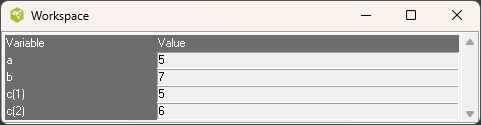
\includegraphics{figures/workspace.png}
\end{example}
\end{document}
